\section{Pendahuluan}
\subsection{Latar Belakang}
Jaringan komputer merupakan komponen utama dalam sistem komunikasi modern karena memungkinkan pertukaran data antar perangkat melalui berbagai jenis media transmisi. Seiring dengan pesatnya perkembangan teknologi, pemahaman mengenai proses perpindahan data dalam jaringan menjadi sangat krusial, khususnya bagi mahasiswa Teknik Komputer. Praktikum Jaringan Komputer dirancang sebagai wadah pembelajaran praktis yang memberikan pengalaman langsung dalam memantau dan menganalisis aktivitas jaringan dengan memanfaatkan beragam alat bantu.

Modul pertama praktikum ini menitikberatkan pada pengenalan serta pemanfaatan Wireshark, sebuah alat analisis protokol jaringan yang banyak digunakan untuk menangkap dan memeriksa paket data yang bergerak di dalam jaringan. Melalui kegiatan ini, mahasiswa diharapkan mampu memahami struktur dasar paket data, mengidentifikasi berbagai protokol komunikasi seperti HTTP, DNS, dan ICMP, serta menganalisis mekanisme kerja pertukaran data secara nyata. Pemahaman tersebut menjadi fondasi penting dalam menguasai aspek teknis jaringan komputer dan keterampilan troubleshooting secara profesional.



\subsection{Dasar Teori}
\subsubsection{Crimping}
Crimping merupakan proses menyambungkan kabel UTP ke konektor dengan bantuan alat crimping guna memastikan transmisi data yang stabil dalam jaringan Ethernet. Tahapan crimping meliputi pengupasan lapisan luar kabel untuk menampakkan kawat tembaga di dalamnya, kemudian menyusunnya sesuai dengan standar pengkabelan yang berlaku. Tujuan utama dari proses ini adalah untuk menjamin setiap kabel terpasang secara tepat pada pin konektor, sehingga aliran data dapat berlangsung tanpa gangguan. Terdapat dua metode utama dalam crimping, yaitu straight-through yang digunakan untuk menghubungkan perangkat berbeda jenis, dan crossover yang diperuntukkan bagi perangkat sejenis.

\subsubsection{Routing IPv4}
Routing IPv4 merupakan proses pengiriman paket data antar jaringan berdasarkan alamat IP versi 4 (IPv4) 32-bit, yang ditulis dalam format desimal bertitik seperti 192.168.1.1, dengan subnet mask seperti /24 yang memisahkan bagian network dan host. Router menggunakan tabel routing, berisi informasi tentang jaringan tujuan, next hop, dan lain-lain. Routing dapat bersifat statis (manual) atau dinamis menggunakan protokol seperti RIP, OSPF, atau BGP, didukung protokol seperti ARP untuk resolusi alamat MAC dan ICMP. Tantangan seperti keterbatasan alamat, fragmentasi, dan risiko keamanan seperti IP spoofing mewarnai proses ini, di mana routing (membangun tabel) berbeda dari forwarding (mengirimkan paket), menjadikannya fondasi penting dalam pengelolaan jaringan.
%===========================================================%
\section{Tugas Pendahuluan}
\begin{enumerate}
	\item tentukan :
    \begin{itemize}
        \item Rentang IP address dan prefix (CIDR) yang sesuai untuk masing-masing departemen.
        \item Total subnet yang diperlukan dan IP network untuk masing-masing departemen 
    \end{itemize}
    Jawaban:

    Rentang IP address dan prefix (CIDR) yang sesuai untuk masing-masing departemen:
\begin{center}
\begin{tabular}{ |c|c|c|c| } 
\hline
Departemen & Perangkat & CIDR & Rentang Ip\\
\hline
Produksi & 50 & /26 & 192.168.0.0 - 192.168.0.63 (64 Ip)\\
Administrasi & 20 & /27 & 192.168.0.64 - 192.168.0.95 (32 Ip)\\
keuangan & 10  & /28 & 192.168.0.96 - 192.168.0.111 (16 Ip)\\
RnD & 100  & /25 & 192.168.0.112 - 192.168.0.239 (128 Ip)\\
\hline
\end{tabular}
\end{center}

  Total subnet yang diperlukan dan IP network untuk masing-masing departemen:
\begin{center}
\begin{tabular}{ |c|c|c|c|c| } 
\hline
Departemen & Subnet & Network address & broadcast\\
\hline
Produksi & 192.168.0.0/26 & 192.168.0.0 & 192.168.0.63  \\
Administrasi & 192.168.0.64/27 & 192.168.0.64 & 192.168.0.95 \\
Keuangan & 192.168.0.96/28 & 192.168.0.96 & 192.168.0.111 \\
RnD & 192.168.0.112/25 & 192.168.0.112 & 192.168.0.239 \\
\hline
\end{tabular}
\end{center}

\item Gambarkan topologi sederhana yang menunjukkan bagaimana router akan menghubungkan semua subnet.
\begin{figure}[h!]
  \centering
  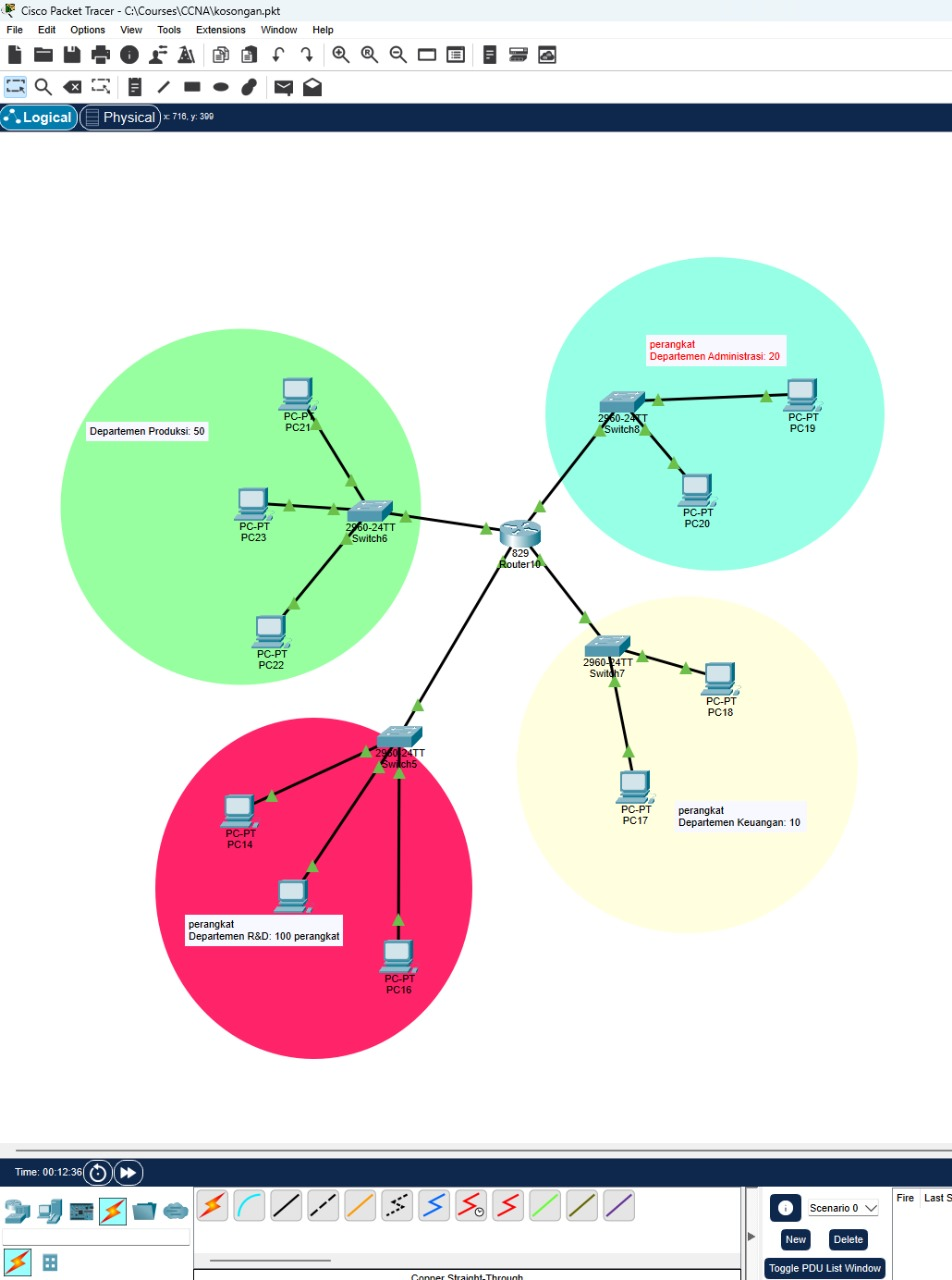
\includegraphics[width=0.5\textwidth]{P1/img/2.jpg}
  \caption{Gambar topologi}
\end{figure}
\item Tuliskan tabel routing sederhana yang menunjukkan:
\begin{itemize}
        \item Network destination
        \item Netmask/prefix
        \item Gateway
        \item Interface tujuan
    \end{itemize}

    Jawab:
    
    Berikut adalah tabel routing yang diperlukan pada router utama:
\begin{center}
\begin{tabular}{ |c|c|c|c|c| } 
\hline
Network Destination & Netmask/Prefix & Gateway & Interface\\
\hline
92.168.0.0/26 & 255.255.255.192 & 92.168.0.1 & eth0  \\
92.168.0.64/26 & 255.255.255.224 & 92.168.0.65 & eth1  \\
92.168.0.96/26 & 255.255.255.240 & 92.168.0.97 & eth2  \\
92.168.0.112/26 & 255.255.255.128 & 92.168.0.113 & eth3  \\
\hline
\end{tabular}
\end{center}

\item Berdasarkan topologi yang telah kamu buat, jenis routing apa yang paling cocok untuk perusahaan ini? Jelaskan alasanmu secara rinci. Pilih salah satu dari opsi berikut (atau lebih jika diperlukan) dan berikan justifikasi mengapa itu menjadi pilihan terbaik untuk perusahaan ini:
\begin{itemize}
        \item Static Routing
        \item Dynamic Routing
        \item CIDR
    \end{itemize}

    jawab:
    Jenis routing yang paling sesuai adalah static routing, mengingat jaringan yang digunakan berskala kecil dengan topologi sederhana yang hanya melibatkan satu router untuk menghubungkan empat subnet. Static routing sangat ideal untuk lingkungan jaringan kecil karena tidak membutuhkan protokol dinamis yang kompleks untuk bertukar informasi antar perangkat. Selain itu, topologi ini telah menerapkan CIDR (Classless Inter-Domain Routing), yang memungkinkan penggunaan alamat IP secara lebih efisien tanpa pemborosan alamat.


\end{enumerate}